\chead{CHAPITRE 2. SPRINT 0 :  ANALYSE ET SPÉCIFICATION DES BESOINS}
 \chapter{Analyse et Spécification des Besoins}
\renewcommand{\mtctitle}{Sommaire}
\minitoc
	\newpage
 \section*{Introduction}
 \addcontentsline{toc}{section}{\protect\numberline{}Introduction}%
Ce chapitre détaille le Sprint 0, phase cruciale d'immersion posant les bases technologiques et fonctionnelles de l'application SmartRec. Il articule l'analyse métier approfondie, la spécification des exigences Salesforce et Heroku, ainsi que la conception de l'architecture cloud intégrée. Sont également exposés le backlog structuré, la modélisation UML des processus de recrutement, la feuille de route Agile et la configuration de l'écosystème de développement SFDX.

\section{Etude du contexte}

L'étude du contexte constitue le pilier de SmartRec, permettant de cartographier l'écosystème de recrutement digital où s'intègre la puissance de Salesforce. Elle définit les attentes précises des recruteurs et candidats, tout en traçant les frontières fonctionnelles entre la gestion des offres et l'automatisation des candidatures. Cette étape assure la viabilité du socle technique, en ancrant chaque cas d'utilisation dans une logique d'optimisation de l'expérience utilisateur et de performance du matching.

\subsection{Identification des acteurs}
Pour appréhender les flux de données et les interactions au sein de SmartRec, il convient de définir précisément les acteurs métiers et leurs périmètres d'action. Le récapitulatif ci-après détaille les privilèges et les responsabilités de chaque profil utilisateur au sein de la plateforme.

 \begin{table}[H]
 \captionsetup{justification=centering}
\caption{Acteurs du système}
\label{tab:acteurs}
\centering
\begin{tabular}{|m{4cm}|m{12cm}|}
\hline 
\centering \textbf{Acteur} & \textbf{Description} \\
\hline Administrateur  & 
Il gère les utilisateurs internes, attribue les rôles, supervise les équipes en désignant les managers, consulte les tâches des employés et accède aux statistiques en temps réel via le tableau de bord.\\
\hline Responsable RH & 
Gère la configuration Salesforce, les habilitations de sécurité, les paramétrages techniques de la plateforme et supervise les tableaux de bord de pilotage global.\\
\hline Recruteur  & 
Pilote le processus de recrutement : création des offres, évaluation des candidatures assistée par les scores de l'IA, gestion des entretiens et sélection des talents.\\
\hline Candidat  &
Utilisateur externe qui postule via le portail dédié, télécharge son CV, gère son profil personnel et suit l’évolution de ses différentes demandes de recrutement.\\
\hline Intelligence Artificielle (NLP)&
Acteur secondaire assurant le parsing automatique des CV (extraction de données) et le calcul du score de matching entre les profils candidats et les offres d'emploi.\\
\hline 
\end{tabular}
\end{table}
\subsection{Spécification des besoins}

La phase de spécification des exigences est capitale pour définir le comportement logique de l'écosystème SmartRec. Elle offre une cartographie précise des fonctionnalités à implémenter sur Salesforce pour garantir une satisfaction optimale des utilisateurs finaux. Cette analyse nous a permis d'organiser les attentes métiers en deux piliers distincts : les besoins fonctionnels et les exigences non fonctionnelles.

\subsubsection{Identification des besoins fonctionnels}
Les besoins fonctionnels détaillent les capacités opérationnelles que SmartRec met à disposition de ses utilisateurs. Ils traduisent les interactions directes que chaque profil peut initier sur la solution Salesforce. Les exigences retenues sont les suivantes :

\hspace{0.5cm}

\begin{itemize}
    \item \textbf{Gestion des accès et des profils utilisateurs :}
    \begin{itemize}
        \item[--]  Les candidats créent leur espace sur le site Experience Cloud pour gérer leur identité et suivre leurs interactions avec l'entreprise.
        \item[--] L'administrateur supervise les comptes des recruteurs, gère les habilitations système et garantit la sécurité des données sur l'organisation Salesforce.
    \end{itemize}
\hspace{0.5cm}

    \item \textbf{Cycle de vie et publication des offres d’emploi:}
\begin{itemize}
    \item[--] Les recruteurs administrent les offres (création, édition, publication) et supervisent leur clôture automatique selon les échéances définies.
     \item[--] Les candidats parcourent l'ensemble des opportunités professionnelles actives publiées sur la plateforme de recrutement.
    \end{itemize} 
\hspace{0.5cm}
    
    \item \textbf{Soumission de candidatures et suivi :}
    \begin{itemize}
        \item[--] Les candidats peuvent postuler aux offres d’emploi via la plateforme.
        \item[--] Ils peuvent suivre le statut de leur candidature (en attente, acceptée ou refusée).
        \item[--] Un système intelligent de tri (scoring automatique) permet de filtrer les candidatures selon leur pertinence.
    \end{itemize}
 \hspace{0.5cm}
    
    \item \textbf{ Dépôt de candidatures et automatisation du tri:}
    \begin{itemize}
        \item[--] Les candidats soumettent leur candidature avec extraction automatique des données de leur CV par l'intelligence artificielle.

        \item[--]Ils visualisent en temps réel l'évolution de leur dossier (À l'étude, Sélectionné ou Refusé) depuis leur espace personnel.

        \item[--] L'IA calcule un score de matching prédictif pour chaque postulant, permettant aux recruteurs de prioriser les profils qualifiés. \end{itemize}

    \end{itemize}
\hspace{0.5cm}

\begin{itemize}
    \item \textbf{GePilotage et supervision de l'activité:}
    \begin{itemize}
        \item[--] Les recruteurs supervisent l'ensemble des candidatures groupées par offre et exploitent les outils de filtrage avancés pour trier les talents.
        \item[--]  L'administrateur surveille la stabilité de la plateforme, les logs système et les statistiques globales de recrutement sur l'organisation.
    \end{itemize}
\hspace{0.5cm}
    
    \item \textbf{Gestion des dossiers et documents:}
    \begin{itemize}
        \item[--] Les recruteurs consultent les dossiers complets des candidats, incluant les CV, les résultats de parsing et les évaluations techniques détaillées.
        \item[--] L'administrateur système garantit l'intégrité des fichiers stockés et gère les autorisations d'accès aux pièces jointes sensibles sur Salesforce.
    \end{itemize}
\hspace{0.5cm}


    \item \textbf{Automatisation et workflow de recrutement:}
    \begin{itemize}
        \item[--] Le système clôture automatiquement les offres dont la date d'échéance est atteinte pour maintenir un catalogue d'opportunités à jour.
        \item[--] Les recruteurs pilotent les étapes du processus, faisant progresser le statut des candidats de l'étude initiale jusqu'à l'embauche finale.
        \item[--]  L'administrateur supervise les processus automatisés pour s'assurer qu'aucun blocage technique n'entrave le flux continu des candidatures.
    \end{itemize}
    
\end{itemize}



\subsubsection{Identification des besoins non fonctionnels}
Afin d'assurer une solution de recrutement robuste, sécurisée et performante sur Salesforce, des exigences non fonctionnelles rigoureuses ont été établies. Elles garantissent la fiabilité technique du système SmartRec et l'optimisation de l'expérience utilisateur.

\hspace{0.5cm}

\begin{itemize}
    \item \textbf{Sécurité et Confidentialité:}
     \begin{itemize}
        \item[--] Protection des données candidats via le modèle de sécurité Salesforce, la gestion fine des profils d'accès et l'authentification Experience Cloud.
    \end{itemize}
\hspace{0.5cm}     

    \item \textbf{Expérience Utilisateur (UX):}
     \begin{itemize}
        \item[--] Interfaces modernes conçues en LWC (Lightning Web Components), offrant une navigation fluide et intuitive pour tous les profils d'utilisateurs.
    \end{itemize}
\hspace{0.5cm}
    \item \textbf{Performance et Réactivité:}
     \begin{itemize}
        \item[--] Optimisation des temps de réponse via l'utilisation du cache client LWC et de traitements asynchrones pour l'analyse des candidatures.
    \end{itemize}
\hspace{0.5cm}
\end{itemize}
\section {Pilotage du projet sous méthodologie SCRUM}
Comme souligné précédemment, la gestion du développement de SmartRec s'appuie sur le framework agile SCRUM. Cette démarche itérative favorise une synergie constante entre les parties prenantes pour livrer une solution Salesforce à haute valeur ajoutée. L'organisation SCRUM retenue s'articule autour de trois piliers fondamentaux :
\vspace{0.3cm}
\begin{table}[H]
\caption{Rôles dans notre projet}
\begin{tabular}{|m{3.5cm}|m{11cm}|}
\hline
\rowcolor{WhiteSmoke} \arrayrulecolor{black}

\hline
\hfil{\cellcolor{WhiteSmoke}\textbf{Role}}
&\hfil{\cellcolor{WhiteSmoke}\textbf{Mission}}\\
 
\hline
\textbf{Product Owner} & Définit la vision produit, priorise le backlog SmartRec et valide l'adéquation des fonctionnalités Salesforce avec les attentes métiers.\\
  \hline

\textbf{Scrum Master} &  Garant du cadre Agile, il lève les obstacles techniques pour assurer la fluidité des sprints et la qualité des livrables de l'application.\\
  \hline
 
\textbf{L’équipe Dev} &  Réalise l'implémentation technique sur Salesforce et Heroku, de la configuration du modèle de données au déploiement des composants LWC.\\
  \hline
\end{tabular}
\end{table}

\section{Backlog produit de SmartRec}

Le Product Backlog constitue le référentiel dynamique des exigences de SmartRec, regroupant les fonctionnalités Salesforce et Heroku à implémenter. Chaque élément — qu'il s'agisse du parsing de CV, du scoring ou de l'interface candidat — est priorisé selon sa valeur métier et sa complexité technique. 
\cite{ScrumOrgBacklog} 
\newline
Il fait office de source de vérité pour l'équipe technique, orientant la planification itérative des sprints de développement. Le Product Owner affine continuellement ces éléments en fonction des retours utilisateurs et des besoins en recrutement, garantissant ainsi un alignement constant avec les objectifs stratégiques du projet.
\cite{AtlassianBacklog} 
\newline
Les principaux attributs de notre backlog:


\begin{itemize}[label=\textbullet]
\item \textbf{ ID } : Identifiant unique permettant la traçabilité de chaque fonctionnalité au sein de l'organisation.
\item \textbf{ User Story} : Expression simplifiée du besoin métier.
\item \textbf{ Priorité } : Niveau d'importance stratégique déterminant l'ordre de traitement dans le flux de développement Agile.
\item \textbf{Sprint} : Itération de travail durant laquelle les fonctionnalités sont conçues, testées et livrées sur l'environnement.\\
\end{itemize}

\begin{table}[H]
\caption{Backlog produit de "SmartRec"}
\centering
\renewcommand{\arraystretch}{1.4}
\begin{tabular}{|p{1.2cm}|p{3.5cm}|p{1.2cm}|p{7.5cm}|p{1.8cm}|}
\hline
\textbf{ID} & \textbf{Fonctionnalit\'e} & \textbf{ID US} & \textbf{User Story} & \textbf{Priorit\'e} \\
\hline

% Administration Salesforce
01 & Administration Salesforce & US 1 & En tant qu'administrateur, je veux configurer les permissions et rôles afin de s'ecuriser les donn'ees RH. & Haute \\
\cline{3-5}
& & US 2 & En tant qu'administrateur, je veux superviser les flux de donn'ees avec le service d'IA (Heroku) pour garantir la stabilit'e. & Haute \\
\cline{3-5}
& & US 3 & En tant qu'utilisateur interne, je veux acc'eder `a des tableaux de bord pour suivre les indicateurs cl'es du recrutement. & Haute \\
\hline

% Espace Candidat
02 & Espace Candidat & US 4 & En tant que candidat, je veux cr'eer un compte sur Experience Cloud pour acc'eder au portail de recrutement. & Haute \\
\cline{3-5}
& & US 5 & En tant que candidat, je veux g'erer mon profil professionnel via l'interface LWC. & Haute \\
\hline

% IA
03 & Analyse de Candidatures & US 6 & En tant que candidat, je veux postuler en t'el'echargeant mon CV pour une extraction automatique de mes donn'ees (Parsing). & Haute \\
\cline{3-5}
& & US 7 & En tant que recruteur, je veux visualiser pour chaque candidat un score de matching calcul'e par l'IA. & Haute \\
\hline

% Gestion du Cycle des Offres
04 & Cycle des Offres & US 8 & En tant que recruteur, je veux publier et modifier des offres d'emploi directement depuis l'organisation. & Haute \\
\cline{3-5}
& & US 9 & En tant que syst`eme, je veux clôturer automatiquement les offres dont la date d''ech'eance est d'epass'ee. & Moyenne \\
\cline{3-5}
& & US 10 & En tant que candidat, je veux consulter et filtrer les opportunit'es professionnelles disponibles en ligne. & Moyenne \\

\hline
\end{tabular}
\end{table}


\begin{table}[H]
\centering
\renewcommand{\arraystretch}{1.4}
\begin{tabular}{|p{1.2cm}|p{3cm}|p{1.2cm}|p{8cm}|p{1.8cm}|}
\hline

% Suivi & Gestion
05 & Suivi et Gestion & US 11 & En tant que candidat, je veux suivre en temps r'eel l''etat d'avancement de mes candidatures. & Moyenne \\
\cline{3-5}
& & US 12 & En tant que recruteur, je veux g'erer les dossiers candidats et consulter les CV via une interface centralis'ee. & Moyenne \\
\hline

% Recrutement intelligent & ATS
06 & Recrutement intelligent & US 13 & En tant que recruteur, je veux utiliser le moteur de matching pour filtrer automatiquement les candidats les plus pertinents. & Moyenne \\
\cline{3-5}
& & US 14 & En tant que recruteur, je veux changer le statut d'une candidature afin de faire progresser le dossier dans le workflow. & Moyenne \\
\cline{3-5}
& & US 15 & En tant que recruteur, je veux acc'eder aux informations d'etaill'ees extraites du CV par l'IA pour 'evaluer le profil. & Moyenne \\
\cline{3-5}
& & US 16 & En tant que recruteur, je veux effectuer des actions group'ees sur les candidatures pour optimiser le traitement des dossiers. & Moyenne \\
\hline

% Gestion des viviers et rapports
07 & Gestion des projets & US 17 & En tant que recruteur, je veux cr'eer des dossiers de talents afin de classer les candidats par type de profil. & Moyenne \\
\cline{3-5}
& & US 18 & En tant qu'administrateur, je veux configurer les crit`eres de matching par d'efaut pour l'intelligence artificielle. & Moyenne \\
\cline{3-5}
& & US 19 & En tant que recruteur, je veux partager une candidature avec d'autres coll`egues pour avis collaboratif. & Moyenne \\
\cline{3-5}
& & US 20 & En tant que recruteur, je veux acc'eder `a l'historique complet des interactions avec un candidat. & Moyenne \\
\cline{3-5}
& & US 21 & En tant qu'administrateur, je veux g'erer les mod`eles d'e-mails automatiques envoy'es aux candidats. & Moyenne \\
\cline{3-5}
& & US 22 & En tant que recruteur, je veux consulter les statistiques de performance des offres publi'ees. & Moyenne \\
\hline

\end{tabular}
\end{table}

\begin{table}[H]
\centering
\renewcommand{\arraystretch}{1.4}
\begin{tabular}{|p{1.2cm}|p{3cm}|p{1.2cm}|p{8cm}|p{1.8cm}|}
\hline

% Expérience Utilisateur & Sécurité
08 & Sécurité et Support & US 23 & En tant que candidat, je veux acc'eder `a une section d'aide afin de comprendre le processus de recrutement. & Basse \\
\cline{3-5}
& & US 24 & En tant que recruteur, je veux archiver les anciennes offres afin de nettoyer la vue op'erationnelle. & Basse \\
\cline{3-5}
& & US 25 &  En tant qu'administrateur, je veux configurer les param`etres de confidentialit'e des donn'ees (RGPD). & Basse \\
\hline

% Maintenance & Personnalisation
09 & Personnalisation  & US 26 & En tant que candidat, je veux r'ecup'erer mon mot de passe en cas d'oubli via une proc'edure automatis'ee. & Basse \\
\cline{3-5}
& & US 27 & En tant que recruteur, je veux personnaliser l'affichage de ma liste de candidatures selon mes pr'ef'erences. & Basse \\
\cline{3-5}
& & US 28 & En tant qu'administrateur, je veux pouvoir activer ou d'esactiver les services d'IA (Parsing/Scoring) & Basse \\
\cline{3-5}
& & US 29 & En tant que recruteur, je veux exporter les donn'ees des candidats retenus pour des besoins de reporting. & Basse \\
\hline

\end{tabular}
\end{table}


\section{Modélisation fonctionnelle : Diagramme de cas d’utilisation generale} 
Le diagramme de cas d'utilisation synthétise les interactions entre les candidats, les recruteurs et l'administrateur avec le cœur de l'application SmartRec. Il expose les fonctionnalités majeures — du parsing de CV au matching intelligent — tout en délimitant les responsabilités et les flux opérationnels de chaque acteur.

\begin{figure}[H]
\centering
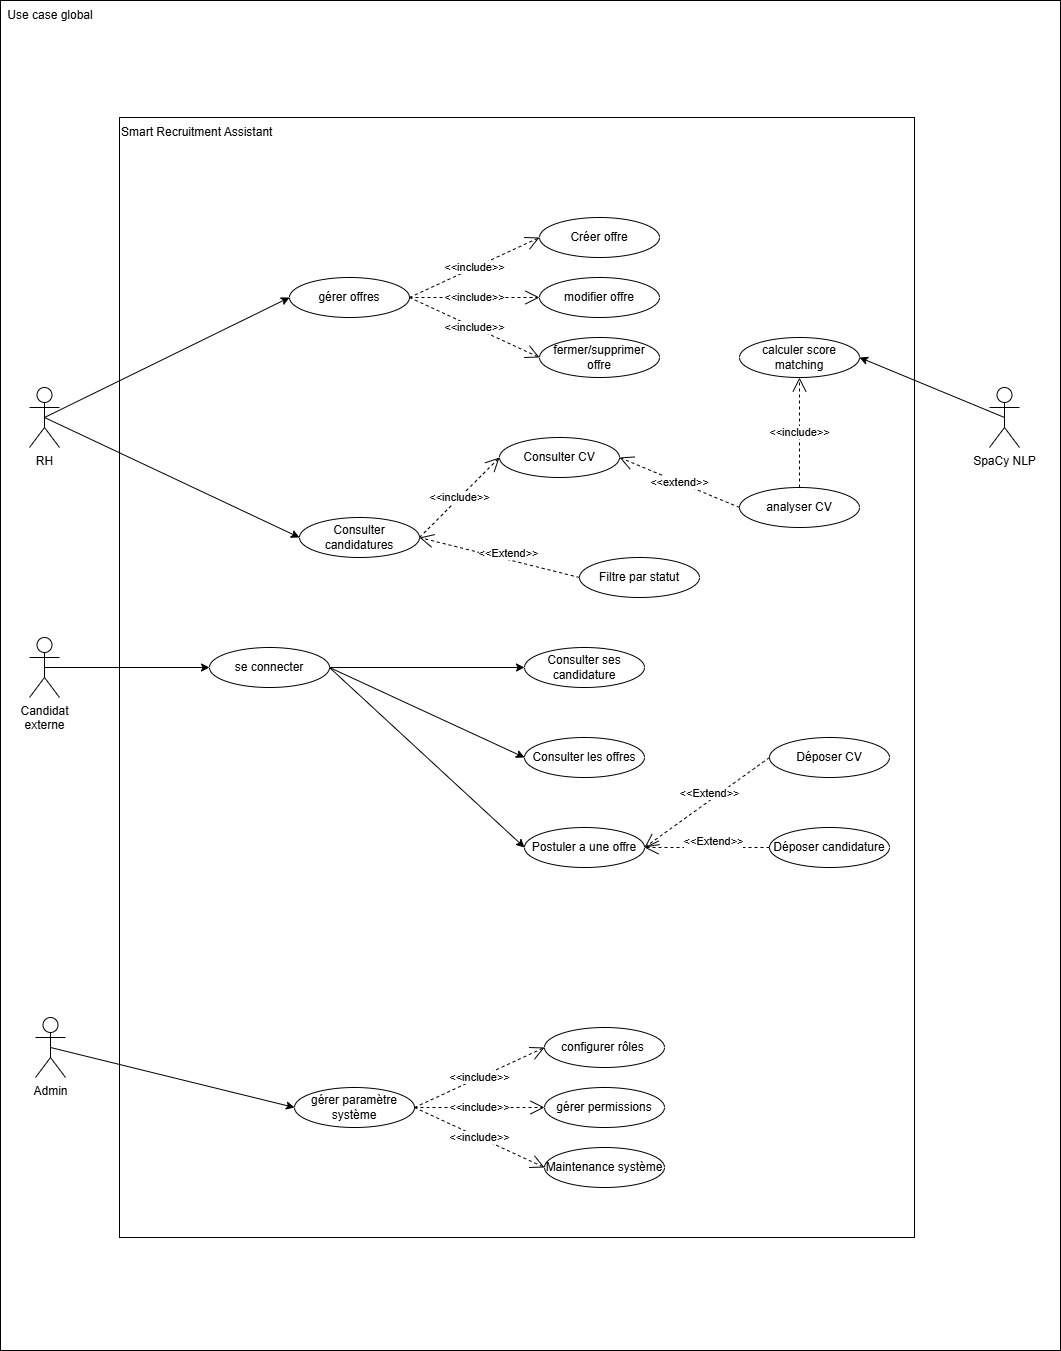
\includegraphics[width=19cm, height=20cm]{Figures/USE case globale.png}
\caption{Diagramme de cas d’utilisation global}
\label{schema1}
\end{figure}
 




\newpage
\section{Conception de la base de données : Diagramme de classes}
Le diagramme de classes structure la modélisation de données de SmartRec, définissant les objets Salesforce (Offre, Candidature, Person Account), 
leurs attributs métiers et les relations d'association. Cette étape est déterminante pour garantir la cohérence du schéma de données et 
l'efficacité des traitements automatisés par les triggers et batchs Apex.

\begin{figure}[H]
\centering

\includegraphics[width=18cm, height=16cm]{Figures/diagramme de classe globale.png'}
\caption{Diagramme de classe global}
\label{schema1}
\end{figure}


\newpage





\section{Feuille de route Agile : Planification des sprints }
Pour garantir une livraison itérative de valeur, le développement de SmartRec a été structuré en 5 sprints distincts. 
Cette organisation repose sur la priorisation du backlog produit, assurant que les socles techniques essentiels précèdent les fonctionnalités de surface.

La réalisation s'est étalée sur une durée de cinq mois, du 2 février au 30 juin 2026. 
Le mois initial a été dédié à l'immersion métier, l'analyse du contexte et la conception technique de l'écosystème Salesforce. 
Le tableau suivant synthétise le cadencement des développements et les objectifs associés à chaque itération.

\vspace{0.3cm}
\begin{table}[H]
\caption{Planification des sprints}
\begin{tabular}{|m{2cm}|m{2.5cm}|m{5cm}|m{6cm}|}
\hline
\rowcolor{WhiteSmoke} \arrayrulecolor{black}

\hfil{\cellcolor{WhiteSmoke}\textbf{Sprint}} &
\hfil{\cellcolor{WhiteSmoke}\textbf{Durée}} &
\hfil{\cellcolor{WhiteSmoke}\textbf{User Stories inclues}} &
\hfil{\cellcolor{WhiteSmoke}\textbf{Objectif du sprint}} \\
\hline

\textbf{Sprint 1} & 4 semaines &
US1, à US5 &
Mise en place de l'organisation Salesforce, gestion des profils/permissions et portail candidat Experience Cloud. \\
\hline

\textbf{Sprint 2} & 4 semaines &
US6, à US8 &
Gestion du cycle de vie des offres d'emploi, publication en ligne et automatisation de la clôture des offres. \\
\hline

\textbf{Sprint 3} & 4 semaines &
US 9 à US 10&
Intégration de l'intelligence artificielle pour le parsing automatique des CV et calcul des scores de matching. \\
\hline

\textbf{Sprint 4} & 4 semaines &
US 11 à US 16  &
Développement du workflow ATS, suivi des candidatures et interface de gestion intelligente pour les recruteurs. \\
\hline

\textbf{Sprint 5} & 4 semaines &
US 17 à US 29   &
Gestion des viviers de talents, tableaux de bord de pilotage, sécurisation RGPD et personnalisation de l'expérience. \\
\hline

\end{tabular}
\end{table}



 \section{ Environnement de développement }
 \hspace{0.5cm}\textbf Le choix d'un écosystème d'outils performants est une étape déterminante pour la réussite du projet SmartRec. Cette section présente l'environnement matériel et les solutions logicielles mobilisés pour la conception et la réalisation de la plateforme.


 
\subsection{Environnement matériel}
Pour assurer la fluidité du développement et la stabilité des outils de build Salesforce, les ressources suivantes ont été utilisées :

\begin{itemize}[label=\textbullet]
\item Ordinateur : Laptop Lenovo haute performance.
\item Processeur : Intel Core Ultra 7, optimisé pour les tâches de compilation.
\item Mémoire vive : 32 Go de RAM pour supporter l'exécution simultanée des IDE et navigateurs. 
\item Système d'exploitation : Windows 11 Famille (Version Unilingue).
\end{itemize}


\subsubsection{Outil de rédaction du rapport}
\hspace{0.5cm}

Le rapport a été rédigé avec \textbf{Overleaf}, un éditeur en ligne basé sur LaTeX, qui permet d’écrire à plusieurs tout en visualisant instantanément le rendu.
Cette plateforme est issue de la fusion entre Overleaf et ShareLaTeX en 2017, donnant naissance à une version améliorée : Overleaf v2., offrant une expérience plus complète et optimisée.
\begin{figure}[H]
\centering

\includegraphics[width=2cm]{ Figures/overleaf-logo.jpg}
\caption{Logo du "LaTeX"}\cite{overleaf_logo}
\end{figure}
\subsubsection{Environnement de développement logiciel}
\hspace{0.5cm}
Pour la réalisation de SmartRec, nous avons exploité l'écosystème Salesforce, complété par des outils de développement modernes assurant agilité et robustesse technique.

\begin{itemize}[label=\textbullet]
\item \textbf{ Salesforce Platform et Apex } :  L'infrastructure cloud fournissant la base de données et 
le langage backend Apex. Ce dernier permet de gérer la logique métier complexe (triggers, batchs) 
de l'application.
\begin{figure}[H]
\centering
\includegraphics[width=2cm]{ Figures/Salesforce_logo.png}
\caption{Logo du  "Salesforce"}\cite{Salesforce_logo}
\end{figure}
\item \textbf{ Lightning Web Components (LWC)} : Le framework UI moderne de Salesforce utilisé pour 
concevoir les interfaces réactives et dynamiques du portail candidat et des outils recruteurs.
\begin{figure}[H]
\centering

\includegraphics[width=2cm]{ Figures/LWC_logo.png}
\caption{Logo du"LWC"}\cite{LWC-logo}
\end{figure}
\item \textbf{ Experience Cloud } : Solution utilisée pour bâtir le site de recrutement externe, permettant aux candidats d'interagir de manière sécurisée avec le système SmartRec. 
\begin{figure}[H]
\centering

\includegraphics[width=2cm]{ Figures/experiencecloud_logo.png}
\caption{Logo du "Experience Cloud"}\cite{experiencecloud_logo}
\end{figure}
\item \textbf{Visual Studio Code} :  Éditeur de code principal, enrichi du "Salesforce Extension Pack". 
Il a permis le développement des composants, l'écriture du code Apex et la gestion des déploiements.
\begin{figure}[H]
\centering

\includegraphics[width=2cm]{ Figures/vs.jpg}
\caption{Logo du "Visual Studio"}\cite{vscode_logo}
\end{figure}
\item \textbf{Salesforce CLI (SFDX) } : Outil en ligne de commande indispensable pour automatiser les déploiements, gérer les environnements et synchroniser le code source avec l'organisation.
\begin{figure}[H]
\centering

\includegraphics[width=2cm]{ Figures/SalesforceCli.png}
\caption{Logo du "Salesforce CLI"}\cite{SalesforceCli}
\end{figure}
\item \textbf{GitHub } : Plateforme de gestion de version utilisée pour centraliser le code source, assurer le suivi des modifications et sécuriser l'historique du développement.
\begin{figure}[H]
\centering
\includegraphics[width=2cm]{ Figures/GitHub_logo.png}
\caption{Logo du "GitHub"}\cite{GitHub-logo}
\end{figure}
\item \textbf{Python } : Utilisé pour développer le moteur d'intelligence artificielle (NLP) hébergé sur Heroku. Il assure le traitement automatique du langage naturel pour extraire les compétences et expériences des fichiers PDF.
\begin{figure}[H]
\centering

\includegraphics[width=2cm]{ Figures/Python-logo.png}
\caption{Logo du "Python"}\cite{python_logo}
\end{figure}
\item \textbf{Apidog } :  Outil utilisé pour tester et documenter les API REST reliant Salesforce au service de parsing. Il a permis de valider la communication et le format des données JSON échangées.
\begin{figure}[H]
\centering

\includegraphics[width=2cm]{ Figures/apidog-logo.png}
\caption{Logo du "Apidog"}\cite{apidog_logo}
\end{figure}
\item \textbf{Draw.io } :  Utilisé pour concevoir les différents diagrammes du projet (classes, cas d’utilisation, architecture), permettant une modélisation claire du système SmartRec.
\begin{figure}[H]
\centering

\includegraphics[width=2cm]{ Figures/draw-logo.png}
\caption{Logo du "Draw.io"}\cite{drawio_logo}
\end{figure}
\end{itemize}



\section{Architecture du système}
\hspace{0.5cm}
La conception architecturale de SmartRec a été pensée pour allier la puissance de la plateforme Salesforce à la flexibilité des services d'IA. Elle définit l'organisation des composants logiciels et leurs protocoles de communication, garantissant ainsi une structure évolutive et sécurisée.

\subsection{Architecture globale de la solution}
\hspace{0.5cm}
 L'architecture de SmartRec repose sur un modèle hybride Cloud-to-Cloud, séparant le portail candidat (Experience Cloud), la gestion métier (Salesforce Core) et le moteur de parsing (Heroku / Python). Cette approche modulaire permet de découpler l'interface utilisateur de la complexité algorithmique du traitement automatique du langage naturel (NLP).

 \begin{itemize}
    \item Une interface utilisateur développée avec les \textbf{Lightning Web Components (LWC)}, sur le portail \textbf{Experience Cloud} pour offrir une expérience fluide et moderne aux candidats.

    \item Un back-end robuste conçu avec le langage \textbf{Apex} au sein de la plateforme Salesforce pour orchestrer la logique métier complexe et les processus automatisés.
    
    \item Une base de données intégrée basée sur les \textbf{Objets Salesforce} (standards et personnalisés), utilisée pour stocker de manière sécurisée les offres, candidatures et profils.

    \item Un microservice indépendant en \textbf{Python}, hébergé sur \textbf{Heroku}, dédié au traitement intelligent (NLP) des CV et au calcul des scores de matching sémantique.
    
\end{itemize}


\hspace{0.5cm}
\begin{itemize}[label=\textbullet]
\item L'interopérabilité entre ces modules est assurée par des API REST sécurisées, garantissant une séparation stricte des responsabilités et une maintenance simplifiée de la solution.

\begin{figure}[H]
\centering
\fbox{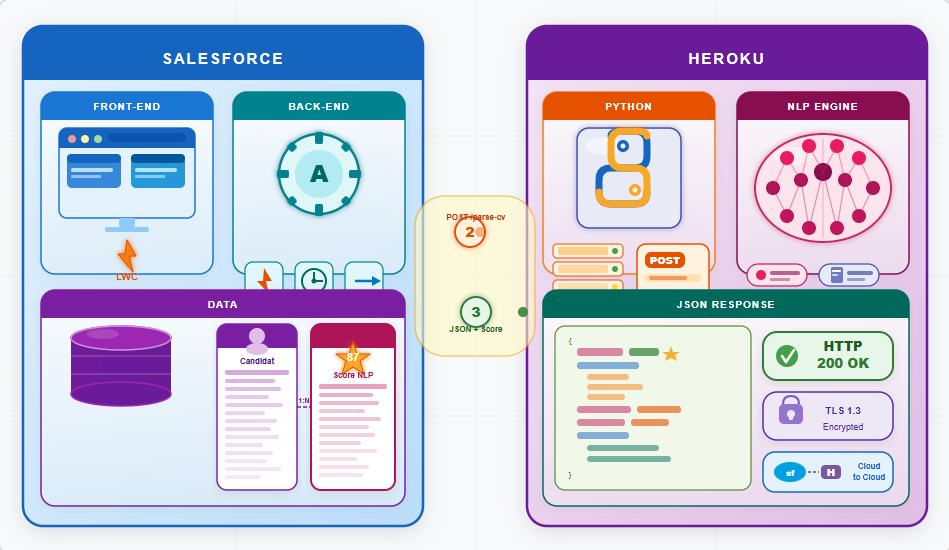
\includegraphics[width=15cm, height=7cm]{Figures/architecture physique.png}}
\caption{Architecture globale}\cite{munonye_microservices_2021}
\label{fig:planification}
\end{figure}



\subsection{Architecture physique}
L’architecture physique décrit la répartition des composants de SmartRec sur les infrastructures cloud et matérielles. Elle illustre la nature distribuée de la solution, garantissant sécurité et scalabilité.

\hspace{0.2cm}
Dans le cadre du projet, l'organisation est la suivante:
\begin{itemize}[label=\textbullet]
\item \textbf{Poste de développement (Local):}Utilisé pour la rédaction du code source (VS Code) et le contrôle de version (Git/GitHub).
\item \textbf{Cloud Salesforce (PaaS) :}Héberge l'interface utilisateur (Experience Cloud), la logique métier (Apex) et le stockage des données (Objets Salesforce).
\item \textbf{Cloud Heroku (PaaS) : }Héberge le microservice Python dédié au traitement NLP des CV, isolant ainsi les tâches de calcul intensif.
\end{itemize}
Les communications entre ces entités s'appuient sur le protocole HTTPS, assurant une transmission cryptée et sécurisée des données sur le réseau internet.
\end{itemize}

\begin{figure}[H]
\centering
\fbox{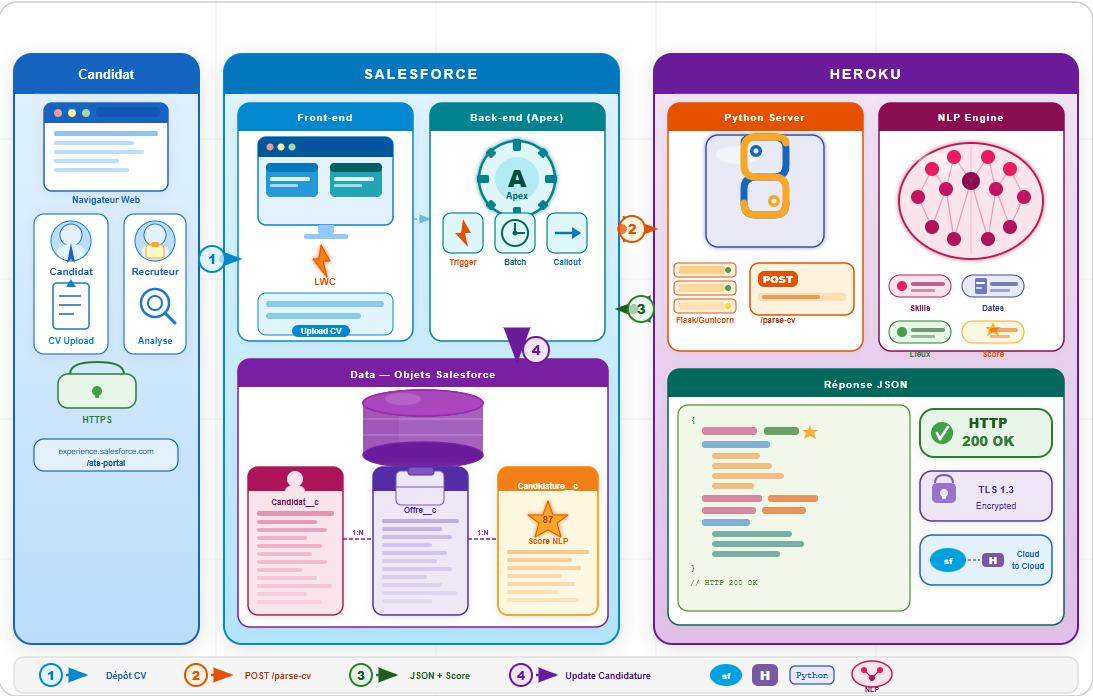
\includegraphics[width=15cm, height=7cm]{Figures/architecture globale.png}}
\caption{Architecture physique}\cite{homedeve_architecture_physique_2023}
\label{fig:planification}
\end{figure}

\subsection{Architecture logique }  
L'architecture logique de SmartRec repose sur le paradigme MVC (Modèle-Vue-Contrôleur), nativement supporté par Salesforce. Cette structure garantit une séparation nette des responsabilités, facilitant la maintenance et l'évolutivité de la solution.
L'application s'articule autour des couches suivantes :
\begin{itemize}[label=\textbullet]
\item \textbf{La Vue (LWC) :}Gère l'interface utilisateur et les interactions dynamiques sur le portail Experience Cloud. 
\item \textbf{Le Contrôleur (Apex) : }Assure la médiation entre l'interface et la base de données, traitant les requêtes envoyées par les composants LWC.
\item \textbf{Le Modèle (Objets Salesforce) :}Définit la structure des données (Offres, Candidatures, Contacts) et assure leur persistance sécurisée.
\item \textbf{La Couche Logique (Triggers et Classes Services) :}Gère les automatisations métier, comme le scoring IA ou les règles de validation anti-doublon.
\end{itemize}
Cette modularité permet de dissocier les traitements complexes de l'interface graphique, assurant ainsi une performance optimale et des tests unitaires simplifiés.

\begin{figure}[H]
\centering
\fbox{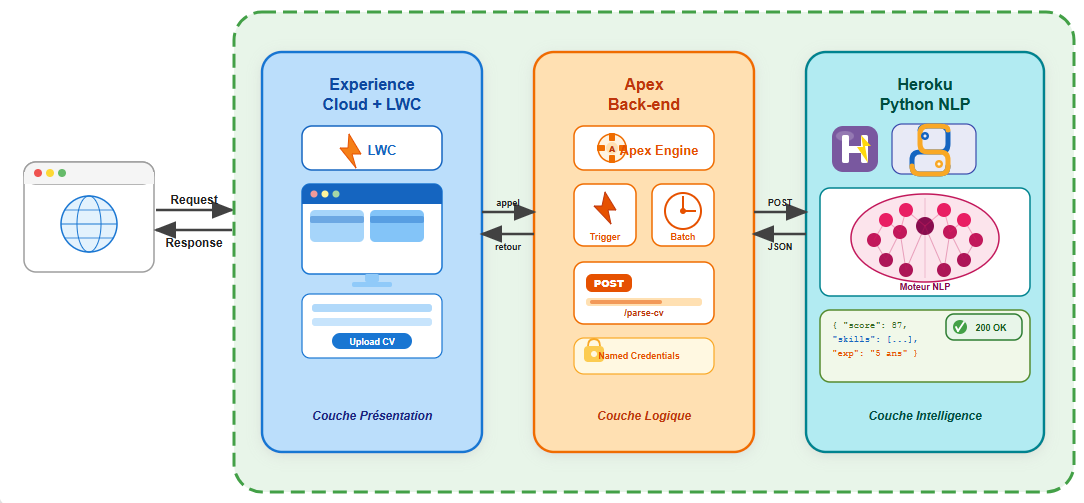
\includegraphics[width=15cm, height=7cm]{Figures/architecture logique.png}}
\caption{Architecture logique}\cite{dyma_springboot_2023}
\label{fig:planification}
\end{figure}

\section*{Conclusion}
Ce chapitre a permis de poser les jalons méthodologiques et techniques indispensables à la réalisation de SmartRec. Nous avons traduit les besoins métiers en spécifications fonctionnelles via le backlog produit et les cas d'utilisation, avant de concevoir une architecture hybride (Salesforce et Heroku) répondant aux exigences de scalabilité. Enfin, la planification détaillée des sprints a été établie pour structurer la phase de développement. Le chapitre suivant sera consacré au premier sprint, dédié à la mise en place du socle de sécurité et à la gestion des accès utilisateurs. 
\addcontentsline{toc}{section}{\protect\numberline{}Conclusion}%
